\section{Introdução}
Em seus primeiros estudos com a acústica, Alexander Graham Bell (1847 – 1922), inventor do telefone, entre outras coisas, percebeu que a variação de som que o ouvido humano pode sentir não acompanha uma escala linear.
Isso significa que se dobrarmos a amplitude de um sinal (duplicar sua tensão elétrica), nosso ouvido não perceberá como sendo o dobro da pressão sonora recebida, ou melhor, o dobro do volume. Graham Bell notou que a escala que o ouvido percebe é logaritma.

Portanto, ao invés de utilizar a escala linear para representar a amplificação (ganho) ou a atenuação (perda) de um sistema, Graham Bell resolveu utilizar uma escala logaritma. Ele verificou, a princípio, que o sinal enviado por um par de fios esticados entre uma cidade e outra, sofria uma grande atenuação (diminuição na amplitude do sinal). Caso estas perdas não fossem corrigidas por meio de amplificadores, o sinal não chegaria inteligível na outra ponta da transmissão.

Graham Bell criou uma unidade de medida para esta atenuação. Esta unidade era chamada originalmente de TU (transmission unit), pelo próprio Graham Bell. Mas em 1929, após a sua morte, os engenheiros do Bell Telephone Laboratory resolveram homenagear seu fundador, dando o nome de Bel (símbolo B) a esta unidade de medida. Por definição do Bell Labs, 1 Bel é igual a atenuação em um sinal de áudio em uma milha (1,61 km) de cabo telefônico. A figura 1 exemplifica esta unidade.

\begin{figure}[hb]
    \centering
    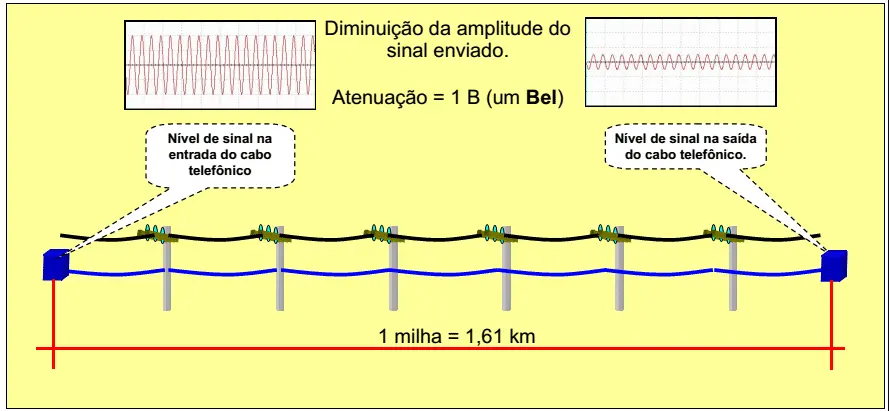
\includegraphics[width=0.6\textwidth]{imgs/bel_e_decibel_unidade.png}
    \caption{Definição do valor de 1 Bel.}
    \label{fig:my_label}
\end{figure}

Com a prática percebeu-se a unidade (1 Bel) era muito grande, ou seja, suas relações resultavam em valores muito elevados. Decidiu-se então dividir a unidade Bel em dez, ou seja, um décimo de Bel. Assim foi criado o Decibel (símbolo dB), como pode ser visto na equação 1.

$$
    \frac{1B}{10}= 1dB \Rightarrow 10dB = 1B
$$

\begin{center}
    Equação 1 – Definição do valor de 1 dB.
\end{center}